\section{Provenance Analysis Methodology}
\label{sec:prop}

\begin{figure*}[!htbp]
\centering
\includegraphics[width=18.4cm]{figures/pipeline2.pdf}
\caption{Proposed pipeline for end-to-end provenance analysis.
The sequence of activities is divided into two parts, which address the tasks of \emph{image filtering} (left panel) and of \emph{graph construction} (right panel).
IVFADC stands for \emph{Inverted File System with Asymmetric Distance Computation}.
RCMM stands for \emph{Reciprocal Condition Matching Measure}.
The value of $n$, within IVFADC, is the number of images in the database.
The value of $k$ is a parameter of the solution and is related to the size of the RCMM rank used for building the provenance graph.
$^\ast$Reported values are merely illustrative.
}
\label{fig:solution}
\end{figure*}

% Preamble
As described in Sec.~\ref{sec:intro}, the task of image provenance analysis is divided into two major steps, namely \emph{Provenance Image Filtering} and \emph{Provenance Graph Construction}.
Fig.~\ref{fig:solution} depicts an overview of the proposed solution in this context.

% This material was already explained above. Cutting for %space. WJS
% Definition of provenance image filtering
%Roughly speaking, provenance image filtering aims at %efficiently and effectively gathering the images that are %related to a target image of interest %(\textit{a.k.a.}~query), from a large image corpus %(\textit{a.k.a.}~gallery, for instance, all the %1.5~million images uploaded to Imgur in the last %day~\cite{imguruploadnumbers}).
%The inherent idea is to retrieve all the gallery images %whose content can be traced back and forward within the %composition history (\textit{a.k.a.}~provenance) of the %query (please refer to Panel~A in Fig.~\ref{fig:teaser} %for a real case example).
%For that, we detail in Sec.~\ref{sec:prop:filtering} the %adopted approach for image filtering, which is %custom-tailored for the provenance task: it extends upon %state-of-the-art efficient image indexing and search %techniques (such as the solution of Johnson et %al.~\cite{johnson2017billion}), by adding novelties such %as \emph{distributed interest point selection} and %\emph{iterative filtering}.
%Such novelties indeed lead to improvements in the final %system retrieval effectiveness, as we further show in %Sec.~\ref{sec:results}.

% Definition of provenance graph construction
%Provenance graph construction, in turn, aims at building %the simple %(in opposition to \emph{multigraph})
%directed acyclic graph whose nodes individually represent %each previously retrieved image or the query itself, and %the edges express the direct content provenance from one %image to the other (please refer to Panel~B in %Fig.~\ref{fig:teaser} for an example).
%For that, in Sec.~\ref{sec:prop:graph_building}, we follow %the literature and first explain how to compute the %dissimilarity matrices, data structures that store the %dissimilarities between every pair of retrieved images.
%In the sequence, we introduce a novel solution for %obtaining the provenance graph from the dissimilarity %matrices, namely \emph{clustered provenance graph %construction}.
%We conclude the issue of Provenance Graph Construction by %introducing graph conciliation techniques that lately %combine different and divergent provenance graphs into a %single and better one.

% Subsections
%\input{./backup/03_prop_01_filtering_joel.tex} (Original)
\subsection{Provenance Image Filtering}
\label{sec:prop:filtering}
The problem of image filtering for the provenance task is different from the typical image retrieval task: a given query image may %simultaneously
fulfill one or both of the following conditions:

\begin{itemize}
    \item The query may have a relationship to various \emph{near duplicates}. The near duplicates may be \emph{hosts} of the query (in the case of the query being a composite that inherits the background from a near duplicate) or the query itself may be a host, as in the case of the query donating a background to the near duplicates.
    
    \item The query may be a composite with a relationship to one or more donors, whose content may be entirely disjoint.
    Donors can even be composites themselves, with their own hosts and donors.
\end{itemize}

In such scenarios, the retrieval method must return as many of the directly and transitively related images as possible.
These aspects define a unique image retrieval and filtering problem, known as \emph{Provenance Image Filtering}~\cite{pinto2017filtering, nist2017plan}, which is different from more typical \emph{near-duplicate} or \emph{semantically similar} image retrieval.
%Therefore, a new system must be designed with the specific purpose of solving such a task.
In this work, we assume that a ground-up system must be deployed for search, retrieval, and filtering, instead of relying on currently available resources such as \emph{Google}~\cite{barroso2003web} or \emph{TinEye}~\cite{jacquicheng}.
%As depicted in Fig.~\ref{fig:solution}, the proposed system starts with a modified interest point selection method (detailed in %Sec.~\ref{sec:prop_spread_kp}), whose output is fed to %a highly-parallelizable
%an image index computation approach inspired by the work in~\cite{johnson2017billion} (detailed in Sec.~\ref{sec:prop_indxing}).
%Once the image indices are obtained, the image search is performed in a way close to~\cite{johnson2017billion} (which is explained in %Sec.~\ref{sec:prop_search}), with the additional step of \emph{iterative filtering} (explained in %Sec.~\ref{sec:prop_iterative_filtering}) that adapts image filtering to the provenance scenario.
%Finally, in Sec.~\ref{sec:prop_scaling}, we explain the strategy to handle millions of images.
 
\vspace{0.2cm} 
\subsubsection{Distributed Interest Point Selection} 
\label{sec:prop_spread_kp}
Due to the nature of the manipulations seen in tampered images, it is important to build a filtering system that is tolerant to a wide range of image transformations.
Hence, we adopt a low-level image representation that is based on interest points and local features, since they are reportedly tolerant to transformations such as scaling, rotation, and contrast adjustment~\cite{Bay:CVIU:2008}.
Nevertheless, while regular interest points are mostly designed to identify corners and blobs on the image, we also want to describe and further index homogeneous areas with low response and consequently a sparse amount of detected interest points, for retrieving images with the same type of content.
Although one can use a dense sampling approach to extract interest points within those regions, this is computationally prohibitive in the context of searching millions of images~\cite{pinto2017filtering}.

Therefore, we introduce a new method called \emph{distributed interest point selection} that aims at keeping a sparse approach while being able to provide interest points inside low-response areas.
For that, we extend Hessian-based detectors (such as Speeded-Up Robust Features (SURF)~\cite{Bay:CVIU:2008}) in the following way.
Instead of employing a threshold $t$ to collect interest points whose local Hessian values are greater than $t$, we define a parameter $p$ that expresses the fixed amount of interest points we want to extract from each target image.
Within these $p$ interest points, $m < p$ interest points are extracted for the reason of being the top-$m$ regions with the $m$ strongest Hessian values.
The remaining $n = p - m$ are extracted from the set containing the post-top-$m$ interest points, which is also sorted according to the Hessian response.
Starting from the $(m+1)$-th strongest interest point, we only add the current interest point if it does not \emph{overlap} with another already selected interest point; otherwise, we try to add the next strongest interest point, up to the point of obtaining $n$ interest points.

\begin{figure}[!t]
\centerline{
    \subfloat[]{\frame{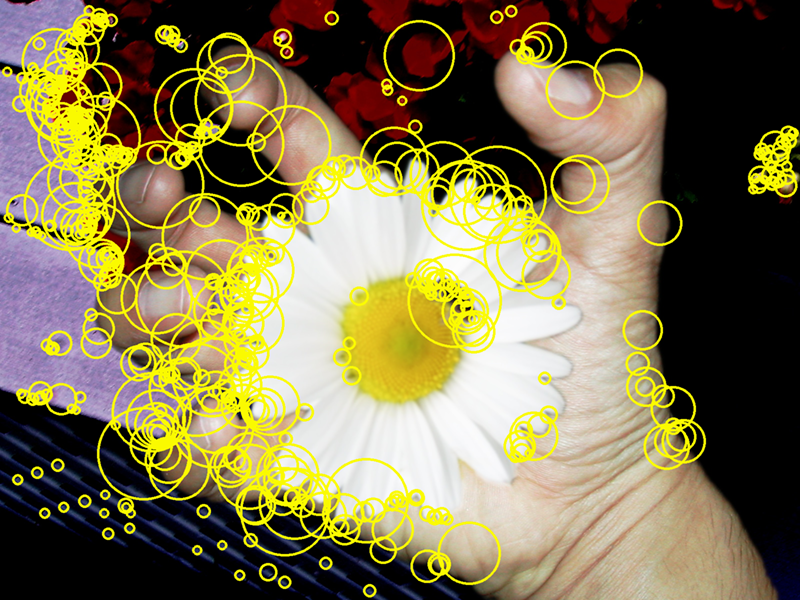
\includegraphics[width=4cm]{figures/rsurf.png}}}
    \hfil
    \subfloat[]{\frame{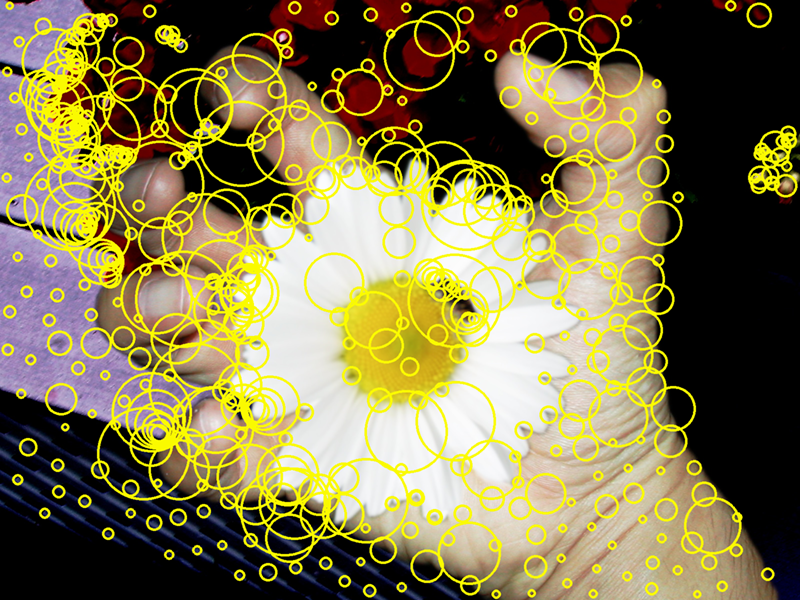
\includegraphics[width=4cm]{figures/dsurf.png}}}
}
\caption{Effects of using the approach of distributed interest point selection.
In (a), the result of a regular SURF interest point detection.
In (b), the result of the distributed approach over the same image, with many more points over homogeneous regions, such as the skin of the wrist.}
\label{fig:disitributed_kp}
\end{figure}

Fig.~\ref{fig:disitributed_kp} depicts the effect of using the distributed approach along with SURF.
Fig.~\ref{fig:disitributed_kp}~(a) depicts a regular SURF detection, while Fig.~\ref{fig:disitributed_kp}~(b) depicts the distributed version, over the same image.
Fig.~\ref{fig:disitributed_kp}~(b) presents more points over the skin of the wrist and background (which are more homogeneous regions) than Fig.~\ref{fig:disitributed_kp}~(a).

%Taking into consideration that each interest point is actually a circular blob with a center $(x, y)$ and a radius $r$, we establish that two points overlap if they do not collide (\textit{i.e.}, they do not share describable content).

\vspace{0.2cm} 
\subsubsection{\RED{Database Indexing}}
\label{sec:prop_indxing}
\RED{The next step is to build the image index structure. %, which we refer to as the CBIR system.
After interest point detection and feature extraction, we are left with $p$ description vectors per image.
For an image collection $C$:}

\begin{equation}
C_i \in C, \quad s.t.\quad  i \in \mathcal{I}_{img} = \{0, 1, \ldots, |C|\},
\end{equation}

\noindent \RED{our subsequent feature collection $F$ is:}

\begin{equation}
F_i \in F, \quad s.t.\quad  i \in \mathcal{I}_{ind} = \{0, 1, \ldots, |C| \times p\},
\end{equation}

\noindent \RED{where $\mathcal{I}_{img}$ denotes the numbered index set of full images within $C$, and $\mathcal{I}_{ind}$ indicates the subsequent numbered index set assigned to individual features in $F$.
We transform $F$ to a new space using \emph{Optimized Product Quantization} (OPQ)~\cite{ge2013optimized} to make the feature space well-posed for coarse \emph{Product Quantization} (PQ).
We refer to this new rotated feature set as $F_{r}$.
From a random sample of $F_{r}$, a coarse set of representative centroids $O$ is generated using PQ.
A subsequent \emph{Inverted File System with Asymmetric Distance Computation} (IVFADC)~\cite{Jegou:TPAMI:2011}) is generated from $O$, allowing for fast and efficient search.}

\vspace{0.2cm} 
\subsubsection{\RED{Image Search}} % and Retrieval}
\label{sec:prop_search}
%Once the CBIR system is built, it can be searched via feature-wise queries.
\RED{Once the database images are indexed, a search procedure can be performed via feature-wise queries.
For a query image $Q$, a set of $p$ distributed SURF features $F_{d}$ is extracted, rotated according to $F_{r}$, and submitted to the system.
Each image $Q$ leads to a matrix of indices of \emph{Approximate Nearest Neighbors} (ANN) $R$ of size $|F_{d}| \times K$, where $K$ is the parameter of the $K$-nearest neighbors for the system to return.
Each $R_{ij}$ value of $R$ is computed using \emph{Asymmetric Distance Computation} (ADC)~\cite{Jegou:TPAMI:2011}:}
\vspace{-0.2cm} 

\begin{equation}
R_{ij}=\mathcal{S}(F_{d_{i}})_{j},\ s.t. \ i \in \{1,...,|F_{d}|\}\ \text{and}\  j \in \{1,...,K\}\,
\end{equation}

\noindent \RED{where $\mathcal{S}$ signifies a feature-wise query search on the IVFADC filtering system, $i$ denotes the $i$-th query feature of $Q$, and $j$ denotes the $j$-th ANN index of the $j$-th nearest feature belonging to $F_{r}$.
As a consequence, each row of $R$ corresponds to a feature in $F_{d}$, containing the $K$-nearest neighbor features, which we may consider as matched features.
We then map $R$ from the $\mathcal{I}_{ind}$ space to the $\mathcal{I}_{img}$ space.
The set of unique related image indices is computed as:}

%\begin{equation}
%\begin{aligned}
%& R_{i,j}=\mathcal{S}(F_{d_{i}})_{j},\ s.t.\\
%& i \in \{0,1,\ldots,|F_{d}|\}\ \text{and}\  j \in K,
%\end{aligned}
%\end{equation}

%\noindent \RED{where $\mathcal{S}$ signifies a single search query on the %CBIR
%filtering system, and $K$ is the parameter of the $K$-nearest neighbors for %the CBIR
%the system to return.
%The set $R$ is subsequently a matrix of size $|F_{d}|*K$, where each row corresponds to a feature in $F_{d}$, containing K nearest neighbor features. We then map $R$ from the $\mathcal{I}_{ind}$ space to the $\mathcal{I}_{img}$ space.
%As a consequence, each row of $R$ corresponds to a feature in $F_{d}$, containing $K$ nearest neighbor features.
%We then map $R$ from the $\mathcal{I}_{ind}$ space to the $\mathcal{I}_{img}$ space.
%The number of unique image indices is computed as:}

\begin{equation}
R_{img}=\mathcal{M}(R,\mathcal{I}_{ind},\mathcal{I}_{img}).
\end{equation}

\noindent \RED{where function $\mathcal{M}(R,\mathcal{I}_1,\mathcal{I}_2)$ maps index values in $R$ from the $\mathcal{I}_{ind}$ domain to the $\mathcal{I}_{img}$ index domain, allowing each $R_{ij}$ to represent the image it belongs to.
Once $R_{img}$ is obtained, a result set of images sorted by the number of matched features is calculated for giving the final global query results of $Q$.}

\RED{The score for each image indexed within $R_{img}$ is therefore denoted by ${freq}(x,R_{img})$, where $x \in \{R_{img}\}$ and ${freq}(x,\cdot)$ is a function that counts the number of occurrences of $x$.}

%The score for each value within ${R_{img}}$ is therefore denoted by the respective tally of feature-wise votes accumulated within $R$.
%Using this scheme, we are able to retrieve images that only partially match $Q$, even in the presence of noisy matches.
%Small local objects will have higher chances of receiving votes than spurious interest points, allowing for burstiness \cite{Jgou2009OnTB}.

%The score for each value within ${R_{img}}$ is denoted by:
%\begin{equation}
%    \mathcal{A}(x,R_{img}),
%\end{equation}

%\noindent where $\mathcal{A}(x,R)$ represents the accumulator that returns the tally of all values of $x$ within $R$.
% \begin{equation}
% \begin{aligned}
%     V_{i} =
%      \begin{cases} 
%       \underset{x \in \{R_{img}\}-V_{i-1}}{\operatorname{argmax}}\{\mathcal{A}(x,R_{img})\}, & \text{if  } i > 0 \\
%       \ \ \ \ \ \ \ \ 0, & \text{if  } i = 0 
%   \end{cases}
% \end{aligned}
% \end{equation}
%Using this scheme, we are able to retrieve images that only partially match $Q$, even in the presence of many noisy matches. Small local objects will have high chances of accumulating values, allowing for burstiness \cite{Jgou2009OnTB} while spurious interest points will not.

\vspace{0.2cm} 
\subsubsection{Iterative Filtering}
\label{sec:prop_iterative_filtering}
Once a first rank of images is retrieved through the search algorithm, we iteratively refine the results to add images that are not directly related to the query, but are still related in some way to its provenance.
%Refer to Fig.~\ref{fig:solution} for an illustration of this process.

In contrast to the approach described by Pinto et al.~\cite{pinto2017filtering}, which employs a two-tiered search to retrieve the small donors of the query after masking the regions that diverge between the query and the first images of the retrieved rank, in this work we employ the \emph{reciprocal condition matching measure} (RCMM) proposed in~\cite{brogan2017spotting} to identify and suppress the near duplicates of the query.
%Given that, the greater the RCMM between two images, the greater the possibility of them being near duplicates, we suppress the retrieved images whose RCMM values with the query are high.
Given that a large RCMM value between two arbitrary images indicates that they are probably near duplicates, we suppress the retrieved images whose RCMM values with the query are large.
% TODO: Daniel: ask Joel more details about this suppression. Is it based on a threshold? Maybe rank position?
The non-suppressed (and therefore non-near-duplicate) images of the current rank are then provided as new queries to the next search iteration, which is performed using the same method explained in Sec.~\ref{sec:prop_search}.

%By applying the above process for a number of iterations, we search various sets of non-near-duplicate queries (which are potentially donors) and end up with a set of ranks, which are then flattened and re-ranked using RCMM.
%In the end, we obtain a less query-centric rank of images, which contains the images directly and indirectly related to the query.
%As we show through experiments in Sec.~\ref{sec:results}, such a strategy improves the recall of the provenance image filtering task, when compared to the application of a regular CBIR system.

By applying the above process for a number of iterations, we search various sets of non-near-duplicate queries (which are potentially donors) and end up with a set of ranks, which are then flattened and re-ranked using RCMM.
In the end, we obtain a less query-centric rank of images, which contains not only images directly related to the query, but also transitively related (\textit{e.g.}, ancestors of the donors of the query).
As will be demonstrated in Sec.~\ref{sec:results}, such a strategy improves the recall of the provenance image filtering task.

% TODO: Daniel: Ask Joel to review the entire following section, including images.
% [MAJOR] Moved to the experimental setup >>>>>>>
%\vspace{0.2cm} 
%\subsubsection{Large-Scale Infrastructure}
%\label{sec:prop_scaling}
%
%Fig.~\ref{fig:filterPipeline} shows the proposed full pipeline for index \emph{training} and \emph{construction} (previously explained in Sec.~\ref{sec:prop_indxing}).
%Index training refers to the process of learning the OPQ rotations and PQ codebooks from a sampling of the local features that are extracted from the target dataset.
%We propose to perform such a step ahead of time with typical central processing units (CPU).
%Index construction, in turn, refers to the computation of the inverted file indices, after properly rotating the previously extracted local features.
%The learning of OPQ rotations and PQ codebooks can be done in advance on a CPU, but the construction of indices is well suited to the capabilities of graphical processing units (GPU), allowing for faster computation.
% TODO: Prof. Rocha's note: Clarify this last sentence. Make it clear what you did in CPU and in GPU.  
%
%\begin{figure}[t]
%\centering
%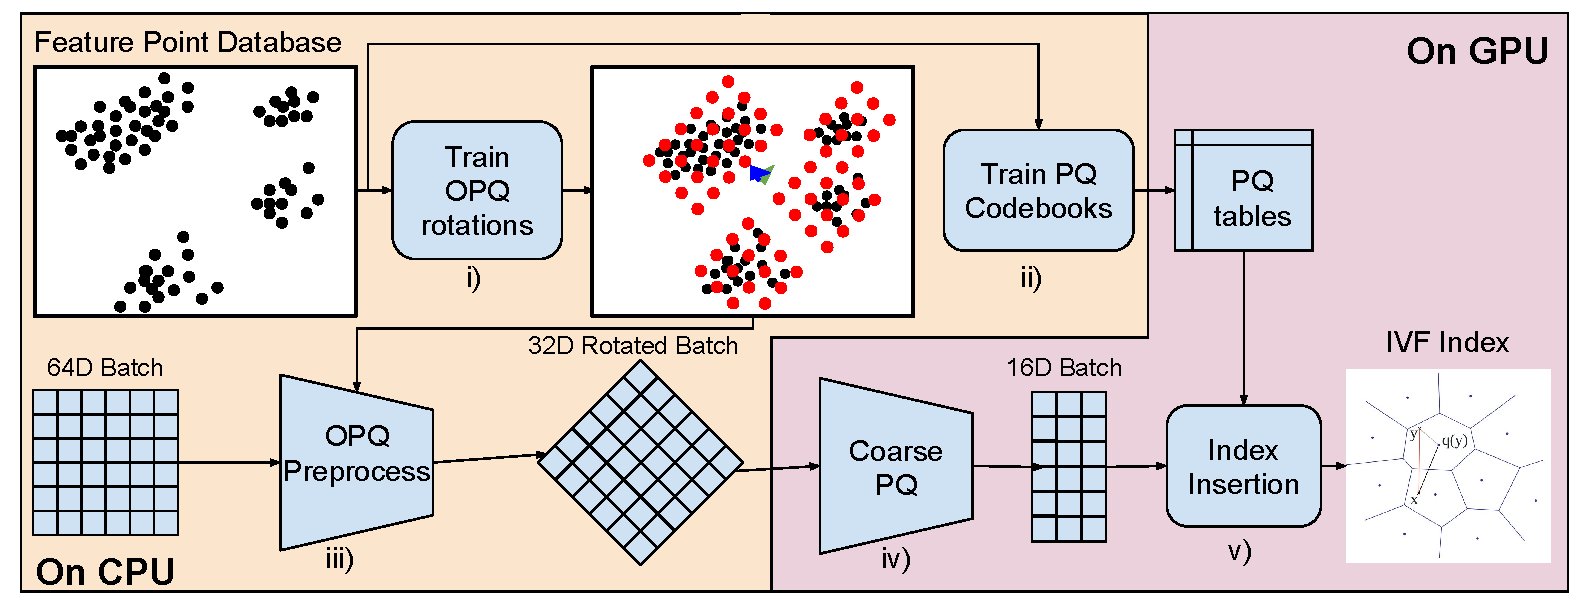
\includegraphics[width=9cm]{figures/Indexing_pipeline.pdf}
%\caption{Filtering pipeline infrastructure.
%The orange area (left) shows computations that are performed on a CPU.
%The purple area (right) shows the index ingestion steps that are performed on a GPU.}
%\label{fig:filterPipeline}
%\end{figure}
% TODO: Prof. Scheirer's note: make on CPU and on GPU labels bold.
%
%\begin{figure}[!htbp]
%\centering
%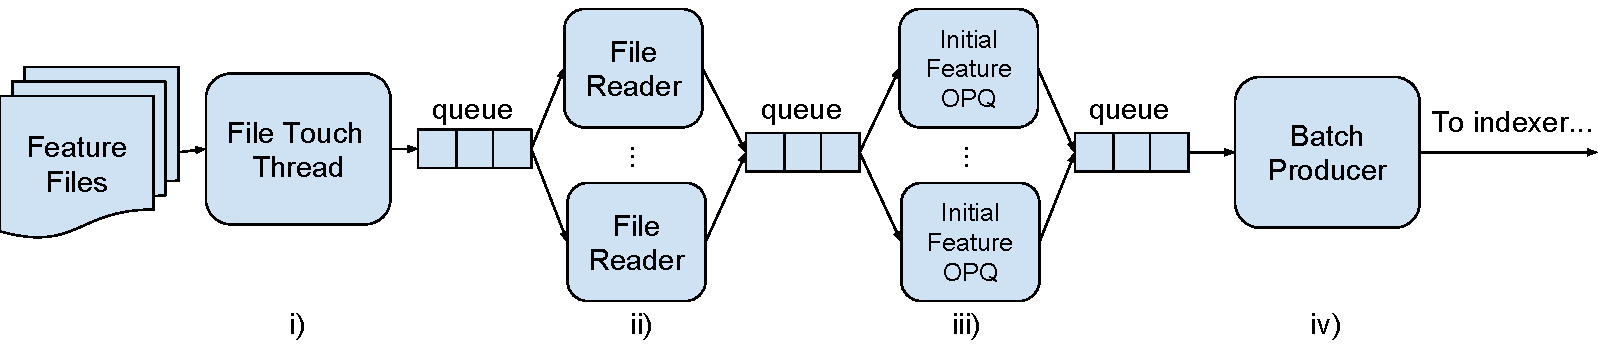
\includegraphics[width=9cm]{figures/Fileread_pipeline.pdf}
%\caption{
%Producer-consumer index ingestion.
%Each file contains features for an image.
%These file locations are pre-loaded into cache via a rate-limited ``touch" thread, and are read on a producer-consumer multi-threaded basis.}
%\label{fig:touchPipeline}
%\end{figure}
% TODO: Prof. Scheirer's note: make image texts larger.
%
%Besides employing GPUs to efficiently build and search an index of over 1 million high-resolution images, additional steps must be taken to increase the pipeline speed.
%To date, most indexing algorithms require singular large files containing all features to be ingested at once \cite{flann_pami_2014,Attach:binary_matching_crv2012}, either due to implementation choices or algorithm limitations.
%The operation of concatenating all features from a set of images into a single file is prohibitively time consuming when dealing with more than a few million interest points.
%Because our scenarios require the ingestion of multiple billions of interest points, a different solution must be adopted, in order to avoid the need for file concatenation.
%For that, we propose a multi-threaded producer-consumer setup, as shown in Fig.~\ref{fig:touchPipeline}.
%In our pipeline, we provide a single feature file per image.
%The pipeline begins with the ``touch" thread, which systematically loads image feature file locations into the computer's file system cache, for faster retrieval in later stages.
%Then, a reading thread takes touched files and loads them into memory.
%A third thread takes sets of loaded feature files and produces feature batches of size $B$ that are optimized in size for GPU ingestion.
%The fourth thread applies the initial OPQ pre-processing rotations to the feature set, before sending the final batch to the GPU. Using this method, we are able to process billions of features from high-resolution image datasets orders of magnitudes faster than previous methods.
% <<<<<<< [MAJOR] Moved to the experimental setup

\subsection{Provenance Graph Construction}
\label{sec:prop:graph_building}

As one can observe in Fig.~\ref{fig:solution}, the provenance graph construction task builds upon the image rank that is obtained by the provenance image filtering task, and ends up with the provenance graph.
Therefore, at this point, we can assume that (in the best scenario) all images directly and transitively related to the query are available for constructing the provenance graph, as well as some \emph{distractors} (images that should not be present in the provenance graph, because they are not related to any of the images within it).

The presence of distractors at this step is more of a matter of design.
Taking into consideration that, in~\cite{bharati2017uphy}, experiments show distractors not impacting the provenance graph construction too much, and aiming to keep the provenance image filtering part as simple as possible, we give the subsequent dissimilarity matrix calculation task the duty of removing distractors. Therefore, the input is a set containing the $k$ top-retrieved images and the query, which are then used for building dissimilarity matrices.

\vspace{0.2cm}
\subsubsection{Calculation of Dissimilarity Matrices}
\label{sec:prop_dismat}
Similar to~\cite{Dias_2012}, given the set $I$ containing the $k$ top-retrieved images and the query, a dissimilarity matrix $D$ is a $(k+1)\times(k+1)$~matrix whose elements $d_{ij}$ describe the dissimilarity between images $I_i$ and $I_j$, respectively the $i$-th and $j$-th images of $I$.
Depending on how the values $d_{ij}$ are calculated, $D$ can be either symmetric or asymmetric.

In this work, following the solution proposed in~\cite{bharati2017uphy}, we neither make any strong assumptions with respect to the transformations that might have been used to generate the elements of $I$, nor impose limitations on the presence of near duplicates, semantically similar images, or multi-donor composites.
Instead, we focus on analyzing the shared visual content between every pair of images $(I_i, I_j)$ through two ways of calculating $d_{ij}$.
In the first one, we set $d_{ij}$ as the inverse of the number of geometrically-consistent interest-point matches (GCM) between images $I_i$ and $I_j$; in this particular case, the matrix $D$ is symmetric.
In the second one, we set $d_{ij}$ as the \emph{mutual information} (MI) between a color transformation $T_j(I_i)$ of image $I_i$ towards image $I_j$; in this case, the matrix $D$ is asymmetric.
Both methods are described below.

\vspace{0.2cm}
\subsubsection*{GCM-based dissimilarity}
%As illustrated in Fig.~\ref{fig:solution},
Provenance graph construction starts with the detection of interest points over each one of the $k+1$ images that belong to $I$.
At this step, different interest point detectors can be applied, such as SURF~\cite{Bay:CVIU:2008} or Maximally Stable Extremal Regions (MSER)~\cite{Matas_2004}, with each one yielding a particular dissimilarity matrix. Once the interest points are available and properly described through feature vectors (\textit{e.g.}, SURF features~\cite{Bay:CVIU:2008}), we find correspondences among them for every pair of images $(I_i, I_j)$.
Let $P_i$ be the set of feature vectors obtained from the interest points of image $I_i$, and $P_j$ be the set of features obtained from $I_j$.
For each feature belonging to $P_i$, the two best matching features are found inside $P_j$ using Euclidean distance (the closer the features, the better the match).
Inspired by Nearest-Neighbor-Distance-Ratio (NNDR) matching quality~\cite{lowe2004distinctive}, we ignore all the features whose ratio of the distances to the first and to the second best matching features is smaller than a threshold $t$, since they might present a poor distinctive quality.
The remaining features are then kept and finally matched to their closest pair.

Even with the use of NNDR, it is not uncommon to gather \emph{geometrically inconsistent matches}, \textit{i.e.}, contradictory interest-point matches that, if together, cannot represent plausible content transformations of image $I_i$ towards image $I_j$, and vice-versa. %, in terms of translation, rotation, and scaling.
%For the sake of illustration, contradictory matches regard the ones that cross each other, as one might observe through the highlighted matches in Fig.~\ref{fig:solution}.
To get rid of these matches, we adopt a solution that is able to build a geometrically-consistent model of expected interest-point positions from any pair of matches between images $I_i$ and $I_j$.
For example, consider two arbitrary matches $m_1$ and $m_2$, which respectively connect points $p_1 \in I_i$ and $q_1 \in I_j$, and points $p_2 \in I_i$ and $q_2 \in I_j$.
Based upon the positions, the distance $l_p$, and the angle $\alpha_p$ between points $p_1$ and $p_2$ (both from image $I_i$), as well as upon the positions, the distance $l_q$, and angle $\alpha_q$ between points $q_1$ and $q_2$ (both from image $I_j$), we estimate the scale, translation, and rotation matrices that make $p_1$ and $p_2$ respectively coincide with $q_1$ and $q_2$.
With these matrices, we transform every matched interest point of $I_i$ onto the space of $I_j$.
As one might expect, points that do not coincide with their respective peers after the transformations have their matches removed from the set of geometrically consistent matches.

% Daniel: I removed the text below to give more space for a better explanation of mutual-information-based solutions.
%Depending on the selected pair of matches for estimating the transformation model, though, different sets of consistent matches may be obtained.
%In this case, one should take the model that returns the set of consistent matches with the largest cardinality (\textit{i.e.}, the maximal set of consistent matches).
%In order to avoid performing an exhaustive search for such a set (by evaluating all the possible pairs of matches between images $I_i$ and $I_j$) we adopt a near-maximal approach, which evaluates only a subset of all the available matches.
%Let $m$ be the total amount of matches established between images $I_i$ and $I_j$, after the application of NNDR.
%After sorting the $m$ matches according to their distances, from the closest to the farthest, we build the mentioned subset with only the $n\leq m$ closest matches.
%With this relaxation, we cannot guarantee that the obtained set of consistent matches is maximal, unless we adopt $n=m$.
%However, there is a big chance of finding the maximal set, since it probably contains at least one of the $n$ best matches.

\RED{Finally, we compute the dissimilarity matrix $D$  by setting every one of its $d_{ij}$ elements as the inverse of the number of found geometrically-consistent matches between images $I_i$ and $I_j$.
In this case, the dissimilarity matrix is symmetric.} %, since $d_{ij}=d_{ji}$.

\vspace{0.2cm}
\subsubsection*{MI-based dissimilarity}
\RED{The mutual-information (MI)-based dissimilarity matrix is  an extension of the GCM-based alternative (see Fig.~\ref{fig:solution}).}
After finding the geometrically consistent interest-point matches for each pair of images $(I_i, I_j)$, the obtained interest points are used for estimating the homography $H_{ij}$ that guides the registration of image $I_i$ onto image $I_j$, as well as the homography $H_{ji}$ that analogously guides the registration of image $I_j$ onto image $I_i$.

In the particular case of $H_{ij}$, for calculating $d_{ij}$, after obtaining the transformation $T_j(I_i)$ of image $I_i$ towards $I_j$, $T_j(I_i)$ and $I_j$ are properly registered, with $T_j(I_i)$ presenting the same size of $I_j$, and the matched interest points relying on the same position.
We thus compute the bounding boxes that enclose all the matched interest points, within each image, obtaining two correspondent patches $R_1$, within $T_j(I_i)$, and $R_2$, within $I_j$.
As in~\cite{bharati2017uphy}, the distribution of the pixel values of $R_1$ is matched to the distribution of $R_2$, prior to calculating the pixel-wise amount of residual between them with MI.

From the point of view of information theory, MI is the amount of information that one random variable contains about another.
From the point of view of probability theory, it measures the statistical dependence of two random variables.
In practical terms, assuming each random variable as respectively the aligned and color-corrected patches $R_1$ and $R_2$, the value of MI is given by the entropy of discrete random variables:
\vspace{-0.2cm}

\begin{equation}
\begin{aligned}
& MI(R_1, R_2) = \\
& \sum_{x \in R_1}^{ }{\sum_{y \in R_2}^{ }{p(x, y)}} \log \left ( \frac{p(x, y)}{\sum_{x}^{ } {p(x, y)} \sum_{y}^{ } {p(x, y)}} \right ),
\end{aligned}
\end{equation}

\noindent where $x \in [0,..,255]$ refers to the pixel values of $R_1$, and $y \in [0,..,255]$ refers to the pixel values of $R_2$.
The $p(x, y)$ value regards the joint probability distribution function of $R_1$ and $R_2$.
As explained in~\cite{Costa_2017}, it can be approximated by:

\begin{equation}
p(x, y) = \frac{h(x, y)}{\sum_{x, y}^{ } {h(x, y)}},
\end{equation}

\noindent where $h(x, y)$ is the joint histogram that counts the number of occurrences for each possible value of the pair $(x, y)$, evaluated on the corresponding pixels for both patches $R_1$ and $R_2$.
As a consequence, MI is directly proportional to the similarity of the two patches.

Back to $H_{ji}$, it is calculated in an analogous way of $H_{ij}$.
However, instead of $T_j(I_i)$, $T_i(I_j)$ is manipulated for transforming $I_j$ towards $I_i$. Further, the size of the registered images, the format of the matched patches, and the matched color distributions are different, leading to a different value of MI for setting $d_{ji}$.
As a consequence, the resulting dissimilarity matrix $D$ is asymmetric, since $d_{ji}\ne d_{ji}$.

\vspace{0.2cm}
\subsubsection*{Avoiding distractors}
As we have mentioned before, the image rank given to the provenance graph construction step may contain distractors, which need to be removed during the dissimilarity matrix calculation step.
When computing the dissimilarity matrix $D$, the solution proposed by Bharati et al.~\cite{bharati2017uphy} establishes matches between every pair of available images, including distractors.
By interpreting $D$ as the adjacency matrix of a multi-graph whose nodes are the images, they identify distractors as the nodes weakly connected (\textit{i.e.,} that present a small number of matches, down to none) to the minimum spanning tree that contains the query.
Assuming $(k + 1)$ as the number of image nodes, they perform $(k^2 + k) / 2$ operations to populate $D$.

In this work, we improve that process by the means of an iterative approach, which starts from the node of the query and then computes the geometrically consistent matches with the remaining $k$ images.
A set with only the strongly connected nodes is thus saved for the next iteration.
In the following iterations, the algorithm keeps trying to establish matches starting from the last set of strongly matched images, up to the point where no more strong matches are found.

Although simple, this solution may provide a significant improvement in the runtime of the dimissimilarity matrix calculation.
Let $d\leq k$ be the amount of distractors inside the image rank.
We avoid $(d^2 - d) / 2$ operations by applying the iterative solution.
In the case of a rank with 50 images ($k=50$), for instance, and 40 distractors ($d=40$) (indicating that the provenance graph contains only ten images), the number of operations is reduced from $1,275$ to $795$, significantly speeding up the runtime in case of small graphs.

\vspace{0.2cm}
\subsubsection{Clustered Provenance Graph Construction}
\label{sec:prop_cluster}
\RED{Once the GCM- and MI-based dissimilarity matrices are available, we rely on both for constructing the final provenance graph, by the means of a novel algorithm, named \emph{clustered provenance graph expansion}. This algorithm, differently from Kruskal's algorithm, delivers directed provenance graphs rather than undirected minimum spanning trees.}

The main idea behind such solution is to group the available images in a way that only near duplicates of a common image are added to the same cluster.
Starting from the image query $I_q$, the remaining images are sorted according to the number of geometrically consistent matches shared with $I_q$, from the largest to the smallest.
The solution then clusters probable near duplicates around $I_q$, as long as they share \emph{enough content}, which is decided based upon the number of matches.
After automatically adding the first image of the sorted set to the cluster of $I_q$, the solution iteratively analyzes the remaining available images.
For deciding if the $i$-th candidate image $I_i$ (where $i>1$) is a near duplicate, the algorithm keeps track of the number of matches $m_i$ between $I_i$ and the last image $I_{i-1}$ added to the cluster.
Let $\mu_{i-1}$ be the average number of matches of the cluster, and $\sigma_{i-1}$ be the standard deviation.
$I_i$ is connected to $I_{i-1}$ in the final provenance graph, if $m_1 \in [\mu_{i-1} \text{ - } \sigma_{i-1}; \mu_{i-1} \text{ + } \sigma_{i-1}]$; in such a case, $I_i$ is added to the cluster by affinity, and novel values of $\mu_i$ and $\sigma_i$ are calculated, for evaluating the next candidate $I_{i+1}$.
Otherwise, the current cluster is considered finished up to $I_{i-1}$.

As a consequence, the obtained clusters have their images sequentially connected into a single path, without branches.
That makes sense in scenarios involving sequential image edits where one near duplicate is obtained on top of the other, as in~\cite{nist2017dataset}.
To determine the direction of a single edge, we rely on the mutual information.
Let $D$ be the MI-based dissimilarity matrix, and consider two images $I_i$ and $I_j$, whose respective $D$ elements are $d_{ij}$ and $d_{ji}$.
As explained in~\cite{Oliveira_2016}, an observation of $d_{ij} > d_{ji}$ means that $I_i$ probably generated $I_j$.

Finally, whenever a cluster is finished and there are still disconnected available images, we find the image already added to the provenance graph whose number of matches with the remaining ones is largest.
This image is then assumed as the new query $I_q'$, over which the aforementioned clustering algorithm is executed, considering only the yet disconnected images.
As a result, the final provenance graph sees a branch rising from $I_q'$ as an orthogonal path containing new images.


% Conclusion of section
%In the following sections, we evaluate the proposed %provenance analysis pipeline, by detailing the %experimental setup (in Sec.~\ref{sec:expsetup}) and %reporting the experimental results over three interesting %datasets (in Sec.~\ref{sec:results}).